
\chapter{The state of the art}

	\section{The introduction of DNS}
	
	Before reading this paper, it is necessary to understand what DNS and TRR are, and what the problem would have in using traditional DNS and why TRR may resolve it.
	
	DNS stands for Domain Name Server. The machines on networks have their own addresses to identify their locations. If users or machines do not have one's address, then they can not connect it or send packets to it.
	
	There are two kinds of addresses, the first one is IP address, which is used for machines to recognize other machines. IP addresses can be IPv4 or IPv6, IPv4 consisted of 4 numbers(0 to 256)\cite{IPv4}, for example 127.0.0.1 is IPv4. IPv6 consisted of 8 numbers(0000 to ffff)\cite{IPv6}, for example 0000:0000:0000:0000:0000:0000:0000:0001 is IPv6. Numbers are easy to be processed by machines, therefore the addresses used by machine consist of numbers.
	
	Contrarily, another kind of addresses is domain name. It consists of several words and is separated by dots, for example, www.tcd.ie is domain name. The words or strings are easy to be remembered by human, thus domain names are mainly used by human\cite{Domain_name}. 
	
	A machine needs a IP address in a network to be recognized by other machines, it can have a domain name to make people to remember it easily, but domain name is not compulsory in a networks. If people type a domain name on their web browser, their computers can translate the domain name into its IP address, then computers use the IP address to search the owner of this IP address in a network.
	
	Hence, it is necessary that having a place to store IP addresses and domain names, moreover, the relations between domain names and IP addresses must be recorded, such as which domain name belongs to which IP address.
	
	That place is so called Domain name server, which is DNS. When users type domain names, their computers use domain names to get correspond IP addresses in a DNS server\cite{what_is_DNS}. 
	
	Moreover, there are 2 kinds of DNS servers, which are recursive DNS resolver and authoritative DNS server. Recursive DNS resolvers do not save all the IP addresses and domain names that users need. If users query the domain names that the recursive DNS resolver does not know, then the recursive DNS resolver will inquire authoritative DNS servers about the IP address for the domain name. After that, the recursive resolver saves the domain name and its IP address in the cache, in case any users use this domain name in a short time, then the recursive resolver is able to reply its IP address immediately and not to inquire authoritative DNS servers again.
	
	About authoritative DNS servers, they store IP addresses and domain names that users need, but users can not inquire them directly, because users have to utilize recursive DNS resolvers to inquire authoritative DNS servers to get correspond IP addresses.
	
	Furthermore, authoritative DNS servers are hierarchical. The highest one is root server. A topper level authoritative DNS server can respond a address of a lower level authoritative DNS server to users for their inquiry, and that lower level authoritative DNS server may have the IP address what users need. In that case, a authoritative DNS server does not need to save entire IP addresses and domain names, the workload can be divided. The levels of authoritative DNS servers are shown in Fig.~\ref{fig:levels_authoritative_DNS_servers}.
	
	\begin{figure}[h]  
    \centering
    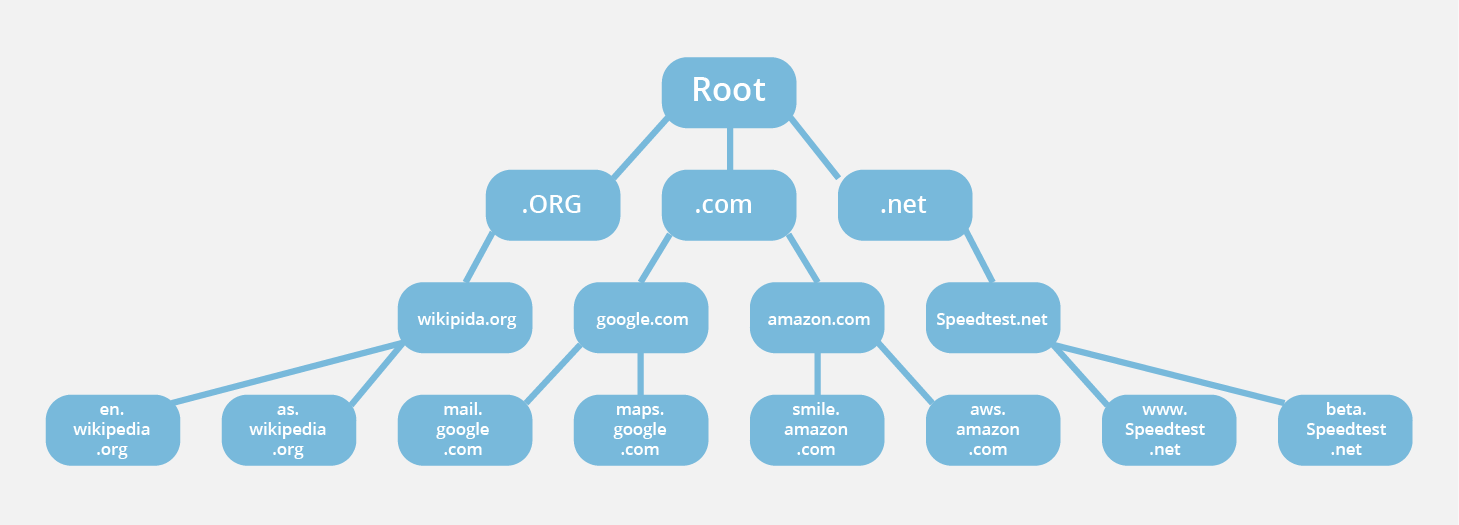
\includegraphics[width=0.8\textwidth]{figure/dns-root-server.png}
    \caption{\em The levels of authoritative DNS servers \cite{dns_root_server_cloudflare}}
    \label{fig:levels_authoritative_DNS_servers}
    \end{figure}
	
	\section{The problem and solutions in using DNS}
	
	DNS servers make people more convenient, but it also has a problem. In using traditional DNS servers, the domain names that users query are not encrypted. Which means, if others get the packets from users, then they can understand what websites users browse or what applications users use.
	
	Wireshark is the software for catching packets in a machine. This study utilized Wireshark to make a small test, when the researcher typed a domain name of a website on a web browser, then that domain name was displayed on Wireshark. The screenshot is shown in Fig.~\ref{fig:traditional_dns_packets}.
	
	\begin{figure}[h]  
    \centering
    \includegraphics[width=0.8\textwidth]{figure/traditional-dns-packets.jpg}
    \caption{\em The queried website is revealed in using a traditional DNS server}
    \label{fig:traditional_dns_packets}
    \end{figure}
    
    Revealing the queried domain name can cause the severe privacy problem. People may not be willing to let others to find what websites they browse. Thus, some solutions were created.
    
    DNSSEC
    
    DOT
    
    DOH
	
	\section{The introduction of TRR}
	
	...
	
	\section{The policy in Ireland}

    ...

    \section{The demand of TRR in Ireland}
    
    ...